% source TeXample.net
% modified Truong Nhan Nguyen

\documentclass[margin=5mm]{standalone}

% preamble
\usepackage{tikz}
\usetikzlibrary{calc, backgrounds}
\usepackage{amsmath, amssymb}

% define picture's scale factor
\def\scala{2.5}
% define tikzstyles
\tikzset{
    background rectangle/.style = {thick, draw=black, fill=white, rounded corners}
}

% body
\begin{document}
    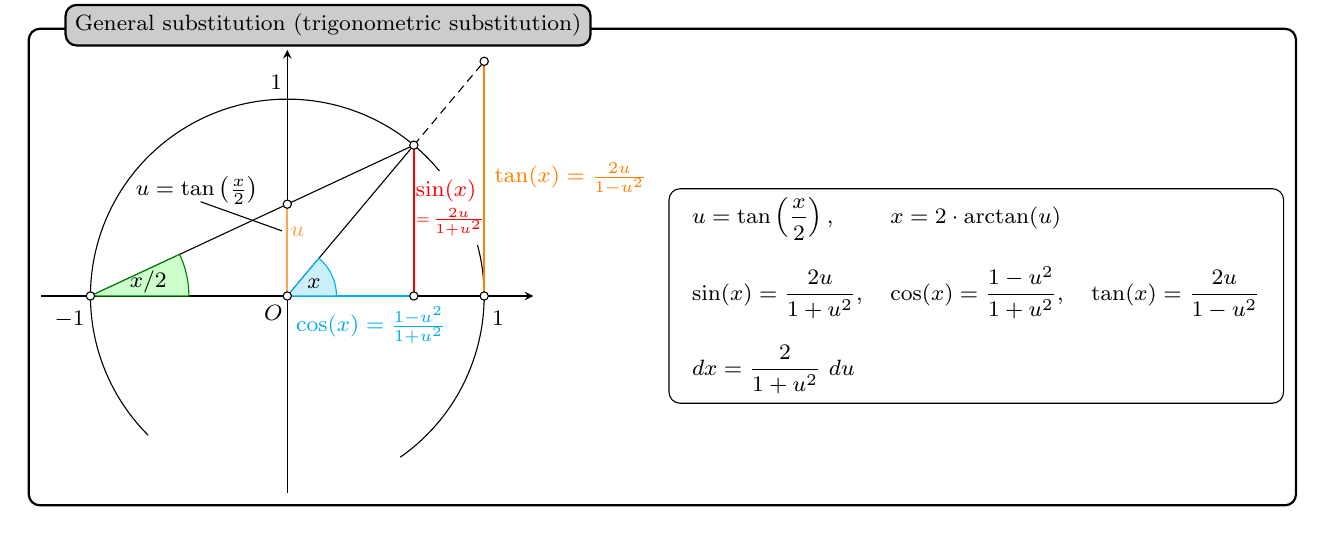
\begin{tikzpicture}[show background rectangle, >=stealth, font=\footnotesize, scale=\scala]
        % specify special coordinates
        \coordinate (O) at (0,0);
        \coordinate (L) at ($({cos(50)},{0})$);
        \coordinate (P) at ($({cos(50)},{sin(50)})$);
        \coordinate (Q) at (-1,0);
        \coordinate (U) at ($({0},{tan(50/2)})$);
        \coordinate (U1) at (-0.5,0.5);
        \coordinate (U2) at ($({0},{tan(50/2)/2})$);
        \coordinate (T) at ($({1},{tan(50)})$);
        \coordinate (F) at (1,0);
        
        % draw trigonometric arc
        \draw[thin] ([shift=(-55:1)]O) arc (-55:225:1);
        
        % draw axe
        \draw[thin, ->] (-1.25,0) -- (1.25,0) node[]{};
        \draw[thin, ->] (0,-1.0) -- (0,1.25) node[]{};
        
        % draw and label sticks
        \draw (1,2pt/\scala) -- (1,-2pt/\scala) node[right=5pt, below]{$1$};
        \draw (-1,2pt/\scala) -- (-1,-2pt/\scala) node[left=7.5pt, below]{$-1$};
        \draw (2pt/\scala,1) -- (-2pt/\scala,1) node[left=2pt, above]{$1$};

        % draw straight lines
        \draw (O) -- (P);
        \draw (Q) -- (P);
        
        % tan (x/2)
        \draw[thick, orange!70] (O) -- (U) node[midway, right, shift={(-2.5pt, 6.5pt)}]{$u$};
        \draw[thin, shorten >=2.0pt, shorten <=4.5pt] (U1) -- ([yshift=2.5pt]U2) node[above=-6pt, pos=0, xshift=3pt]{$u = \tan\left(\frac{x}{2}\right)$};
        
        % cosine line
        \draw[thick, cyan] (O) -- (L) node[midway, below, xshift=7.5pt]{$\cos(x)=\frac{1-u^2}{1+u^2}$};
        
        %sine line
        \draw[thick, red] (P) -- (L) node[fill=white, align=left, midway, right=-3pt, yshift=4.5pt]{$\sin(x)$ \\ \tiny$=\!\frac{2u}{1+u^2}$};
        \draw[thick, red] (P) -- (L);
        
        % tang line
        \draw[thick, orange] (T) -- (F) node[midway, right]{$\tan(x) = \frac{2u}{1-u^2}$};
        
        %dashed line
        \draw[densely dashed] (P) -- (intersection of 0, 0 -- P and 1, 0 -- 1, 1);
        
        % x angle
        \filldraw[thin, fill=cyan!20, draw=cyan] (0, 0) -- (0.25, 0) arc (0:50:0.25) --cycle;
        \draw (25:0.15) node {$x$};
        
        % x/2 angle
        \filldraw[thin, draw=green!50!black, fill=green!20] (Q) -- (-0.5, 0) arc (0:25:0.5) node[xshift=-0.4cm,yshift=-0.35cm]{$x/2$} -- cycle;

        %\draw[very thin] ([shift=(205:0.4)]P) arc (205:230:0.4) node[xshift=0.15cm, yshift=0.4cm]{$\varrho$};
        %\draw[<->, very thin] ([shift=(50:0.25)]O) arc (50:180:0.25) node[xshift=0.0cm, yshift=0.5cm]{$\chi$};

        % % right angle
        % \draw[thin] ([shift=(90:0.15)]L) arc (90:180:0.15) node[xshift=0.25cm, yshift=0.1cm]{\Large$\cdot$};
        
        % mark special points defined before
        \filldraw[fill=white] (O) circle (1.5pt/\scala) node[left=5pt, below]{$O$};
        \filldraw[fill=white] (L) circle (1.5pt/\scala);
        \filldraw[fill=white] (P) circle (1.5pt/\scala);
        \filldraw[fill=white] (Q) circle (1.5pt/\scala);
        \filldraw[fill=white] (U) circle (1.5pt/\scala);
        \filldraw[fill=white] (T) circle (1.5pt/\scala);
        \filldraw[fill=white] (F) circle (1.5pt/\scala);

        \node[draw, rounded corners] at (3.5,0) {$%
            \begin{array}{lll}
                u = \tan\left(\dfrac{x}{2}\right), & x = 2 \cdot \arctan(u) & \\ \\
                \sin(x) = \dfrac{2u}{1+u^2}, & \cos(x) = \dfrac{1-u^2}{1+u^2}, & \tan(x) = \dfrac{2u}{1-u^2} \\ \\
                dx = \dfrac{2}{1+u^2} ~ du
            \end{array}
        $};

        \node [xshift=2ex, yshift=-0.5ex ,overlay, thick, draw=black, fill=lightgray!80, rounded corners, above right] at (current bounding box.north west){General substitution (trigonometric substitution)};

    \end{tikzpicture}
\end{document}